\documentclass{article}
%%%%%%%%%%%%%%%%%%%%%%%%%%%%%%%%%%%%%%%%%%%%%%%%%%%%%%%%%%%%%%%%%
\usepackage[a4paper]{geometry}
\geometry{left=3cm,right=3cm,top=3cm,bottom=3cm}
\linespread{1.5}
\usepackage{fancyhdr}

\usepackage{fontspec}
\defaultfontfeatures{Mapping=tex-text}
\usepackage{xunicode,xltxtra}
\usepackage[BoldFont,SlantFont,CJKnumber,CJKchecksingle]{xeCJK} \usepackage{CJKfntef}
\usepackage{bm} 
\usepackage{pifont}
\usepackage{color,xcolor}
\definecolor{GREEN}{RGB}{25,180,68}
\definecolor{YELLOW}{RGB}{255,255,224}
\definecolor{BLUE}{RGB}{65,105,225}
\definecolor{RED}{RGB}{139,0,0}
\definecolor{DRED}{RGB}{128,0,0}
\definecolor{GREY}{RGB}{128,128,128}

\usepackage{amsmath,amsfonts,amssymb}

\usepackage[americaninductors,europeanresistors]{circuitikz}
\usepackage{tikz}
\usetikzlibrary{positioning,arrows,shadows,shapes,calc,mindmap,trees,backgrounds}
\usepackage{graphicx}
\usepackage{subfigure} 
\usepackage{colortbl,dcolumn}  
\usepackage{multirow}
\usepackage{multicol}
\usepackage{booktabs}
\usepackage{fancyvrb}
\usepackage{listings}

\usepackage{titlesec}
\usepackage{etoolbox}
\makeatletter
\patchcmd{\ttlh@hang}{\parindent\z@}{\parindent\z@\leavevmode}{}{}
\patchcmd{\ttlh@hang}{\noindent}{}{}{}
\makeatother
\usepackage{mdwlist}
\usepackage{verbatim}
\usepackage{/Users/jinna/styles/zhfontcfg}
\usepackage{/Users/jinna/styles/visionouclistings}
\usepackage{/Users/jinna/styles/visionouccfg}
\setlength{\headheight}{15pt}
\fancyhf{}
\makeatletter
\def\headrule{{\if@fancyplain\let\headrulewidth\plainheadrulewidth\fi%
\color{BLUE}
\hrule\@height 2.5pt \@width\headwidth\vskip1pt 
\hrule\@height 0.5pt\@width\headwidth              
\vskip-2\headrulewidth\vskip-1pt}        
\vspace{6mm}}                
\makeatother         

\graphicspath{{figures/}}
\tikzset{
    >=stealth',
    punkt/.style={
           rectangle,
           rounded corners,
           draw=black, very thick,
           text width=6.5em,
           minimum height=2em,
           text centered},
    pil/.style={
           ->,
           thick,
           shorten <=2pt,
           shorten >=2pt,},
    FlyZhyBall/.style={
      circle,
      minimum size=6mm,
      inner sep=0.5pt,
      ball color=red!50!blue,
      text=white,},
    FlyZhyRectangle/.style={
      rectangle,
      rounded corners,
      minimum size=6mm,
      ball color=red!50!blue,
      text=white,},
    zhyfly/.style={
      rectangle,
      rounded corners,
      minimum size=6mm,
      ball color=red!25!blue,
      text=white,},
    nrectangle/.style={
      rectangle,
      draw=#1!50,
      fill=#1!20,
      minimum size=5mm,
      inner sep=0.1pt,}
}

% code
\lstnewenvironment{VHDLcode}[1][]{%
  \lstset{
    basicstyle=\footnotesize\ttfamily\color{black},%
    columns=flexible,%
    framexleftmargin=.7mm,frame=shadowbox,%
    rulesepcolor=\color{blue},%
%    frame=single,%
    backgroundcolor=\color{yellow!20},%
    xleftmargin=1.2\fboxsep,%
    xrightmargin=.7\fboxsep,%
    numberstyle=\tiny\color{blue},%
    numberblanklines=false,numbersep=7pt,%
    language=VHDL%
    }\lstset{#1}}{}
\lstnewenvironment{VHDLmiddle}[1][]{%
  \lstset{
    basicstyle=\scriptsize\ttfamily\color{black},%
    columns=flexible,%
    framexleftmargin=.7mm,frame=shadowbox,%
    rulesepcolor=\color{blue},%
%    frame=single,%
    backgroundcolor=\color{yellow!20},%
    xleftmargin=1.2\fboxsep,%
    xrightmargin=.7\fboxsep,%
    numbers=left,numberstyle=\tiny\color{blue},%
    numberblanklines=false,numbersep=7pt,%
    language=VHDL%
    }\lstset{#1}}{}
\lstnewenvironment{VHDLsmall}[1][]{%
  \lstset{
    basicstyle=\tiny\ttfamily\color{black},%
    columns=flexible,%
    framexleftmargin=.7mm,frame=shadowbox,%
    rulesepcolor=\color{blue},%
%    frame=single,%
    backgroundcolor=\color{yellow!20},%
    xleftmargin=1.2\fboxsep,%
    xrightmargin=.7\fboxsep,%
    numbers=left,numberstyle=\tiny\color{blue},%
    numberblanklines=false,numbersep=7pt,%
    language=VHDL%
    }\lstset{#1}}{}
% pdf
\hypersetup{pdfauthor={Haiyong Zheng},%
            pdftitle={Title},%
            CJKbookmarks=true,%
            bookmarksnumbered=true,%
            bookmarksopen=false,%
            plainpages=false,%
            colorlinks=true,%
            citecolor=green,%
            filecolor=magenta,%
            linkcolor=DRED,%red(default)
            urlcolor=cyan}
\newcommand\titlebar{%
\tikz[baseline,trim left=3.1cm,trim right=3cm] {
    \fill [cyan!25] (2.5cm,-1ex) rectangle (\textwidth+3.1cm,2.5ex);
    \node [
        fill=cyan!60!white,
        anchor= base east,
        rounded rectangle,
        minimum height=3.5ex] at (3cm,0) {
        \textbf{\thesection.}
    };
}%
}

\definecolor{mygreen}{rgb}{0,0.6,0}
\definecolor{mygray}{rgb}{0.5,0.5,0.5}
\definecolor{mymauve}{rgb}{0.58,0,0.82}
\lstset{
 backgroundcolor=\color{white}, 
 basicstyle = \footnotesize,       
 breakatwhitespace = false,        
 breaklines = true,                 
 captionpos = b,                    
 commentstyle = \color{mygreen}\bfseries,
 extendedchars = false,             
 frame =shadowbox, 
 framerule=0.5pt,
 keepspaces=true,
 keywordstyle=\color{blue}\bfseries, % keyword style
 language = C++,                     % the language of code
 otherkeywords={string}, 
 numbers=left, 
 numbersep=5pt,
 numberstyle=\tiny\color{mygray},
 rulecolor=\color{black},         
 showspaces=false,  
 showstringspaces=false, 
 showtabs=false,    
 stepnumber=1,         
 stringstyle=\color{mymauve},        % string literal style
 tabsize=2,          
 title=\lstname                      
}


%%%%%%%%%%%%%%%%%%%%%%%%%%%%%%%%%%%%%%%%%%%%%%%%%%%%%%%%%%%
%设置标题页面               
\chead{\color{GREY}Research Progress}%页眉
\cfoot{\color{GREY}12.13}%页脚 中
\lfoot{\color{GREY}Jinna}%页脚 左
\rfoot{\color{GREY}\thepage\ }%页脚 右
\renewcommand{\headrulewidth}{0.4pt}
\renewcommand{\footrulewidth}{0.4pt}
\usepackage{/Users/jinna/styles/lshort}

%%%%%%%%%%%%%%%%%%%%%%%%%%%%%%%%%%%%%%%%%%%%%%%%%%%%%%%%%%%%%%%%%
\begin{document}

\pagenumbering{roman}


\pagestyle{fancy}
%%%%%%%%%%%%%%%%%%%%%%%%%%%%%%%%%%%%%%%%%%%%%%%%%%%%%%%%%%%%%%%%%
\begin{center}
\textbf{\LARGE{ICIP Papers Research Progress}} %标题加黑加大居
\end{center}

\begin{center}
Jinna Cui
\end{center}

\begin{center}
12.04 - 12.11
\end{center}
\section{Research Dataset}
My database is WHOI - Plankton database which contains 103 classes and about 3.6 millions images. I set the images collected in 2006 - 2013 as training database, and images collected in 2014 as test database. The classes and amount of training database and test database are showed in table 1. The reason why test database is just 95 classes is that 8 classes of images collected in 2014 are empty. They are: Bacillaria, Bidulphia, bubble, Gonyaulax, Hemiaulus, Karenia, Strombidium\_wulffi, Tiarina\_fusus, Tontonia\_appendic\_ulariformis. 

\begin{table}[!ht]
  \caption{Research Dataset}
  \centering
  \begin{tabular}{lllll}
    \toprule
    \cmidrule{1-3}
    Category     &Classes      &Amount \\
    \midrule
    train\_dataset & 103   & 3.2 million \\ \hline
    test\_dataset & 95   &0.3 million   \\
    \bottomrule
  \end{tabular}
\end{table}

\section{Research Evaluating Indicator}
\textbf{\large{Classification Overall Accuracy:}}
\[
classification\ overall\ accuracy =  \frac{The\ amount\ of\ correct\ classified\ images}{The\ amount\ of\ all\ images}
\]
I mainly focus on the overall accuracy of classifier and ignore the precision of each class. So, the classification overall accuracy is main evaluating indicator, a model with higher classification means more effective classifier. I aim to get higher and higher classification overall accuracy. Besides, the loss value is a reference.
\section{Research Benchmark}
My method of plankton classification is based on original CNNs, such as Cifar10, AlexNet, VGG16 and so on.  As 3-channel AlexNet works better than 3-channel Cifar10, and VGG16 is too slow to train, so I choose AlexNet as main benchmark to test the effectiveness of different feature acquire methods during my feature-acquirement-methods-testing stage. After finding out the best method, I will try training on VGG16, and ResNet, and the other new types CNNs, such as Inception V4.
\begin{figure}[!ht] 
  \centering 
  \subfigure[Structure]{ 
    \label{fig1} %% label for first subfigure 
    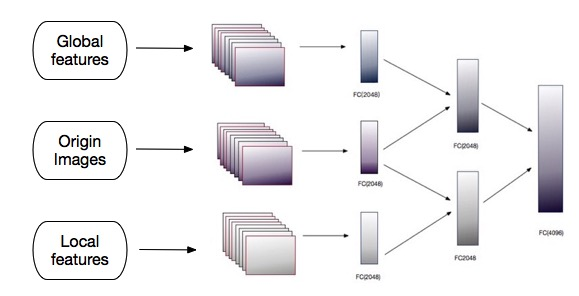
\includegraphics[width=14cm,height=8cm]{1}} 
  \hspace{0.3in} 
\end{figure}

My benchmark is training original images of our database on original CNNs to get the overall accuracy. After that, I need use my methods to acquire effective features and extend the convolution part (including convolution layer, pooling layer and Activation function layer) into three channels (showed in fig. a). After that, trained original images, global feature images and local feature images to trained on 3-channel CNNs to get the overall accuracy again. Finally, compare these two accuracies. Till now, I have got two benchmarks (AlexNet and VGG16):
\begin{table}[!ht]
  \caption{Benchmarks}
  \centering
  \begin{tabular}{lllll}
    \toprule
    \cmidrule{1-3}
    category     &max\_iter      &highest\_accuracy\_iter    &accuracy\\
    \midrule
    AlexNet &200000   &55980 &93.58\% \\ \hline
    VGG16 &200000   &104000 &94.89\%   \\
    \bottomrule
  \end{tabular}
\end{table}
\section{Research Method}
We can see in figure(a) that, the global features and local features are vital. In the research, I mainly focus on acquiring effective global features and local features. As you can see in the following two figures, I aim to acquire effective global feature which means clear boundary which contains shape information without inside details and effective local feature which means clear and bright inside textures. To achieve this, my plan is as follows:

Firstly, I plan to change another enhancement method since logarithmic enhancement doesn't work well (verified by experiment, the accuracy after logarithmic enhancement didn't increase too much), I plan to try other enhancement methods. 
 
Secondly, I plan to find out whether there are some enhancement methods can process the global feature images that can enhance the boundary. 

Thirdly, I plan to try other methods to obtain global features and local features. 

Finally, because the quality of original images is low, I wonder whether I can do enhancement to original images, such as histogram enhancement to get clear texture in dark parts of images.

\begin{figure}[!ht] 
  \centering 
  \subfigure[Global Features Acquirement]{ 
    \label{fig1} %% label for first subfigure 
    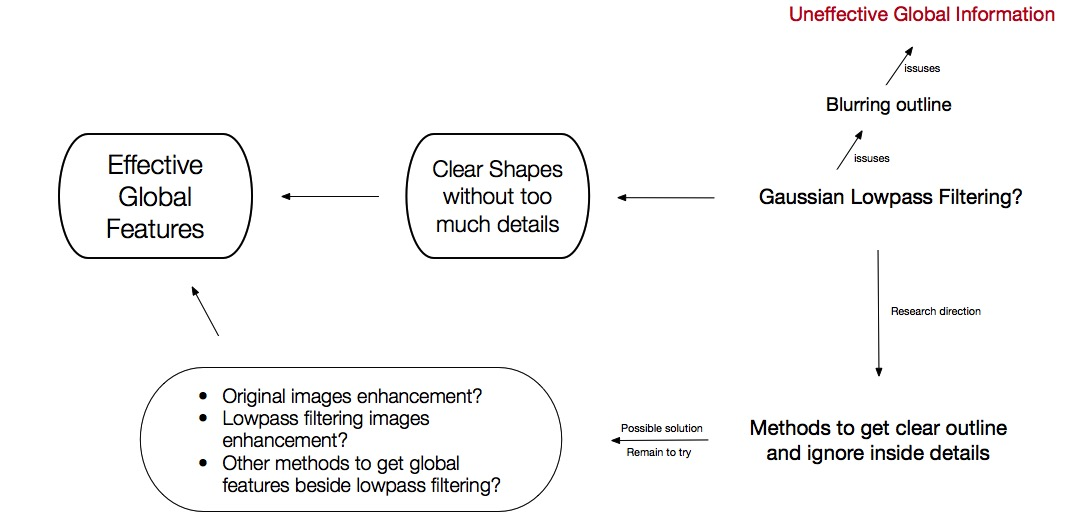
\includegraphics[width=14cm,height=7cm]{global}} 
  \hspace{0.3in} 
\end{figure}

\begin{figure}[!ht] 
  \centering 
  \subfigure[Local Features Acquirement]{ 
    \label{fig1} %% label for first subfigure 
    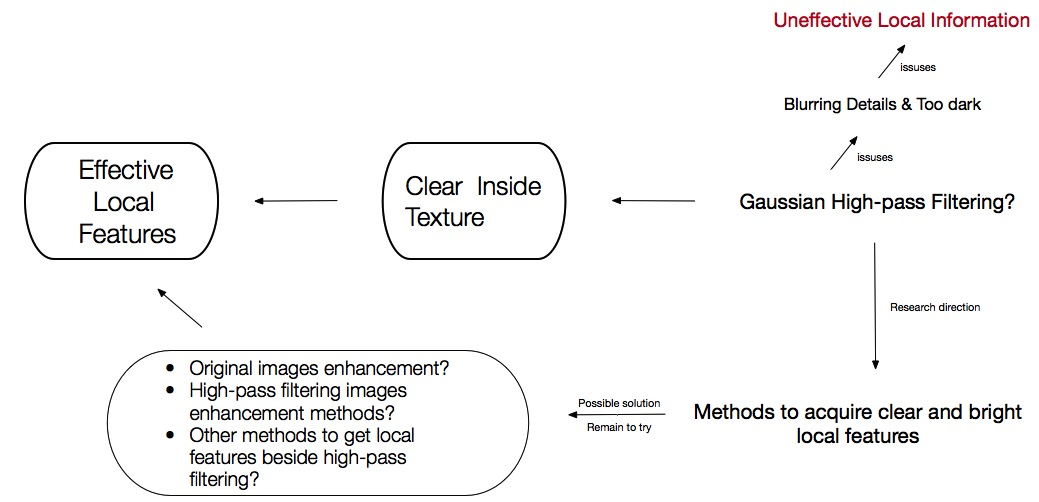
\includegraphics[width=14cm,height=7cm]{local}} 
  \hspace{0.3in} 
\end{figure}

\end{document}